\documentclass[a4paper, 12pt]{article}%тип документа



%отступы
\usepackage[left=1cm,right=1cm,top=1cm,bottom=2cm,bindingoffset=0cm]{geometry}

%%% Работа с русским языком
\usepackage{graphicx}
\usepackage{cmap}                           % поиск в PDF
\usepackage{mathtext} 			 	       % русские буквы в формулах
\usepackage[T2A]{fontenc}               % кодировка
\usepackage[utf8]{inputenc}              % кодировка исходного текста
\usepackage[english,russian]{babel} 
\usepackage{float}

\usepackage[export]{adjustbox} % локализация и переносы

\usepackage{subfig}% http://ctan.org/pkg/subfig
\usepackage{booktabs}

\usepackage{wrapfig}


%Матеша
\usepackage{amsmath,amsfonts,amssymb,amsthm,mathtools} % AMS
\usepackage{icomma} % "Умная" запятая

%\mathtoolsset{showonlyrefs=true} % Показывать номера только у тех формул, на которые есть \eqref{} в тексте.

%% Шрифты
\usepackage{euscript}	 % Шрифт Евклид
\usepackage{mathrsfs} % Красивый матшрифт

%% Свои команды
\DeclareMathOperator{\sgn}{\mathop{sgn}}

%% Перенос знаков в формулах (по Львовскому)
\newcommand*{\hm}[1]{#1\nobreak\discretionary{}
	{\hbox{$\mathsurround=0pt #1$}}{}}


%\usepackage{caption}
%\usepackage{subcaption}

\date{18 октября 2022 г.}
\author{Гаврилин Илья Дмитриевич \\
	Б01-101}
\title{\textbf{Работа 3.1.1 \\ 
		Магнитометр}}
	
\begin{document}
	\maketitle
	\section{Аннотация}
	В данной работе определили горизонтальную составляющую магнитного поля Земли (если точнее значение данного поля в окрестности установки с учетом поправок окружающей среды). Установили качественное соотношение между единицами электрического тока в системах СИ и СГС.
	\section{Теоретические сведения}
	\begin{figure}[H]
		\centering
		\subfloat[Элементы установки]{{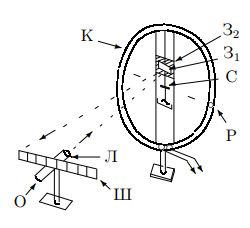
\includegraphics[width=0.478\textwidth]{установка}}}
		\qquad
		\subfloat[Схема измерения угла]{{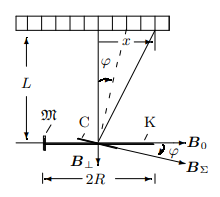
\includegraphics[width=0.478\textwidth]{угол}}}
		\caption{Оборудование для проведения эксперимента}
	\end{figure}
	Поле намагниченного стержня (поле диполя) на перпендикуляре к нему:
	\begin{equation}
		B_1 =\frac{\mu_0}{4\pi} \frac{M}{R^3}
	\end{equation}
	поле в центре кольца с током по закону Био и Савара:
	\begin{equation}
		B_2 =\frac{	\mu_0I}{2R} N
	\end{equation}
	Здесь
	$M$ — магнитный момент ферромагнитного стержня,
	$R$ — радиус кольца,
	$N$ — число витков в кольце,
	$I$ — сила тока в единицах СИ (амперах).
	Измерив угол отклонения стрелки	$\phi$, можно связать поля
	$B_0$ и $B_\perp$ ($B_1$ или $B_2$):
	\begin{equation}
		B_\perp =B_0 \cdot tg(\phi)
	\end{equation}
	\begin{center}
		\textbf{I. Определение горизонтальной составляющей магнитного поля Земли}
	\end{center}
	Для определения горизонтального земного поля $B_0$ тонкий и не очень длинный намагниченный стержень
	устанавливается в отверстие Р на горизонтальном диаметре кольца (рис. 1). Измерив угол отклонения стрелки $\phi_1$
	\begin{equation}
		tg(\phi_1) = \frac{x_1}{2L}
	\end{equation}
	можно с помощью уравнений (1), (3)
	и (4) рассчитать поле $B_0$, если исключить величину $M$ — магнитный момент стержня.
	Исключить магнитный момент можно, измерив период крутильных
	колебаний стержня в поле Земли. Подвешенный горизонтально за середину на
	тонкой длинной нити стержень в положении равновесия
	установится по полю Земли (упругостью нити можно пренебречь). Если ось стержня отклонить в
	горизонтальной плоскости от направления
	$B_0$ на малый угол
	$\alpha$, то под действием возвращающего механического момента
	\begin{equation*}
		M_{мех} = M B_0 sin(\alpha) \approx M B_0 \alpha
	\end{equation*}
	стержень с моментом инерции
	$J$ в соответствии с уравнением
	\begin{equation*}
		J \ddot{a} + M B_0 \alpha = 0
	\end{equation*}
	будет совершать крутильные колебания c периодом
	\begin{equation}
		T = 2 \pi \sqrt{\frac{J}{MB_0}}
	\end{equation}
	Момент инерции цилиндрического стержня относительно оси вращения
	\begin{equation}
		J = m (\frac{l^2}{12} + \frac{r^2}{4}) = \frac{ml^2}{12}(1 + 3( \frac{r}{l})^2)
	\end{equation}
	где
	$m$
	— масса стержня, $l$ — длина,
	а $r$ — его радиус.
	Таким образом, рассчитав момент инерции
	и измерив угол отклонения
	стрелки
	$\phi_1$ и период малых крутильных
	колебаний стержня
	$T$, можно с помощью формул (1), (3), (4)
	и (5) определить горизонтальное поле:
	\begin{equation}
		B_0 = \frac{2 \pi}{TR} \sqrt{\frac{\mu_0 JL}{2\pi R x_1}}	
	\end{equation}
	Поскольку магнитометр
	установлен в железобетонном здании, магнитное поле в нём может не только сильно отличаться от поля Земли, но
	и заметно
	меняться от места
	к месту, поэтому период
	колебаний следует определять
	вблизи магнитометра. Для
	устранения случайных помех стер
	жень подвешивается в специальном стеклянном сосуде.
	\begin{center}
		\textbf{II. Определение электродинамической постоянной}
	\end{center}
	Для определения электродинамической постоянной c необходимо провести независимые измерения одного
	и того же тока в разных системах: в СИ—$I_{СИ}$
	и в абсолютной гауссовой — $I_{абс}$:
	\begin{equation}
		c = 10 \frac{[I]абс}{[I]СИ}
	\end{equation}
	Пропуская ток через витки магнитометра, измеряют тангенс угла отклонения
	стрелки и по формулам (2)
	и (3) рассчитывают величину
	\begin{equation}
		I_{СИ} = \frac{2B_0 R}{\mu_0 N} tg(\phi_2) = A tg(\phi_2)
	\end{equation}
	Величина
	$A$ является постоянной прибора в данном месте земной поверхности.
	Заметим, что если $B_0$ известно, то определение силы тока не требует сравнения с какими-либо эталонами тока или напряжения
	и является абсолютным, т.е. непосредственно связывает ток с основными единицами системы СИ. При этом магнитометр может служить для изготовления эталонов
	и
	градуировки амперметров в системе СИ.
	\begin{equation}
		I_{абс} = CUn
	\end{equation}
 \section{Ход работы}
 1. Включили осветитель, настроили схождение двух световых зайчиков на линейке, настроили их четкость путем фокусировки.\\
 2. Установили магнит разными полюсами и замерили отклонение луча:\\
 $x_0 = +7.5 \pm 0.1$ см, $x_1 = -5 \pm 0.1$ см, $x_2 = +20.5 \pm 0.1$ см, тогда для отклонения в разные стороны получаем: $\Delta x_+ = 13 \pm 0.1$ см,  $\Delta x_- = 12.5 \pm 0.1$ см. Отклонение составляет <5\% значит можно продолжать опыт.\\
 3. Замерили расстояние от линзы для измерительной линейки: $L = 93\pm 0.2$ см.\\
 4. Замерим период малых вращательных колебаний магнитного стержня:\\
 $t = 61.4 \pm 1$ сек., $N = 37$, значит $T = 1.66 \pm 0.03$ сек.\\
 5. Замерим линейные размеры магнитного стержня: $d = 4.5 \pm 0.1$ мм, $l = 24.0 \pm 0.1$ мм, $m = 2.87 \pm 0.01$ гр.\\
 6. Рассчитаем момент инерции магнита (по ф-ле 6): \\
 \begin{equation}
 	J = \frac{ml^2}{12}(1 + 3( \frac{r}{l})^2) = (1.41 \pm 0.05) \cdot 10^{-7}~ кг\cdot м^2
 \end{equation}
 7. Рассчитаем $B_0$ по формуле (7):\\ 
 \begin{equation*}
 	\varepsilon_{B_0} = \sqrt{\varepsilon_{T}^2+\frac{9}{4}\varepsilon_{R}^2 + \frac{1}{4}\varepsilon_{J}^2 + \frac{1}{4}\varepsilon_{L}^2+ \frac{1}{4}\varepsilon_{x}^2}
 \end{equation*}
 \begin{equation*}
 	B_0 = \frac{2 \pi}{TR} \sqrt{\frac{\mu_0 JL}{2\pi R \Delta x_+}}= (1.47 \pm 0.08) \cdot 10^{-5} ~Тл
 \end{equation*}
 7.\textbf{Собрали электрическую схему для сравнения значений токов.}\\
 8.Рассмотрим отклонение зайчика при разной полярности источника:\\
 $x_0 = +7.5 \pm 0.1$ см, $x_1 = -5 \pm 0.1$ см, $x_2 = +20.5 \pm 0.1$ см, тогда для среднее отклонение зайчика: $\Delta x = 12.75 \pm 0.25~ см$.\\
 При этом напряжение на конденсаторе было равным: $U_c = 96~В$\\
 Параметры установки: $R_{резистор} = 1.2 ~кОм$, $С = 9 \cdot 10^5 ~м$, $N = 34~витка$.\\
 9. Замерим $x_2$ и $U$ на вольтметре подсчитаем токи по формулам (9) и (10).
 \begin{equation*}
 		I_{СИ} = \frac{2B_0 R}{\mu_0 N} tg(\phi_2) = (0.023 \pm 0.004) А
 \end{equation*}
 \begin{equation*}
	I_{абс} = CUn = (28.8\pm 0.16) \cdot 10^6 ~ед.СГС
 \end{equation*}
\begin{equation}
	c = 10 \frac{[I]абс}{[I]СИ} = (2.6 \pm 0.6) \cdot 10^{10}~см/с
\end{equation}
\section{Выводы}
1. Измерили горизонтальную составляющую магнитного поля Земли: 	$B_0 = (1.47 \pm 0.08) \cdot 10^{-5} ~Тл$. Для Москвы горизонтальную составляющую можно принять за $2 \cdot 10^{-5} ~Тл$, однако на это значение влияет множество побочных факторов: экранирование металлоконструкциями, наводимые проводкой поля. Поэтому, полученное значение можно назвать значением магнитного поля в окрестности лабораторной установки. \\
2. Определили связь между единицами тока в СГС и СИ, получили значение скорости света в СГС. Наше значение: $	c  = (2.6 \pm 0.6) \cdot 10^{10}~см/с$, а эталонное: $	c = 3 \cdot 10^{10}~см/с$. Получили значение совпадающее с теоретическим в пределах погрешности.
\end{document}